% Research plan, Helmholtz Munich AIH PI call. Build: latexmk -xelatex research_plan.tex  (or ./build/render.sh)
\documentclass[11pt,a4paper]{article}
\usepackage[margin=2cm]{geometry}
\usepackage{fontspec}\setmainfont{Times New Roman}
\usepackage[super,sort&compress,comma]{natbib}
\usepackage{graphicx,booktabs,float,caption,titlesec,etoolbox,multicol}
\usepackage[hidelinks]{hyperref}
\titleformat{\section}{\normalfont\fontsize{11.5}{13}\bfseries}{}{0em}{}
\titlespacing*{\section}{0pt}{6pt plus 2pt}{2pt}
\captionsetup{font=small,labelfont=bf,skip=3pt}
\setlength{\parskip}{2.5pt}\setlength{\parindent}{0pt}
\renewcommand{\baselinestretch}{0.97}
\setlength{\bibsep}{0pt}
\renewcommand{\bibsection}{\section*{References}}
\newcommand{\plantitle}[1]{{\fontsize{13}{15}\bfseries #1\par}\vspace{4pt}}
\pagestyle{plain}
\begin{document}
\plantitle{What if, and why: tissue representations one can intervene on, interpret and test}

A cell's response to a drug or a mutation depends on the tissue around it. Predicting that response \emph{in silico} is the promise of perturbation models and of the foundation models trained on hundreds of millions of single cells. That promise has not held up to simple tests: on unseen perturbations, linear baselines match or beat specialist and foundation models alike \citep{ahlmanneltze2025linear, wu2024perturbench}. In our perspective on the field \citep{dimitrov2026interpretation}, we argued that the failure often comes from the data rather than the architectures: these models learn from dissociated cells, which offer only partial views of causality, because the microenvironmental cues that shape a cell's response were never measured. Spatial foundation models now embed hundreds of millions of cells together with their neighbourhoods \citep{blampey2025novae, tejadalapuerta2025nicheformer, birk2026terra, wenckstern2026virtues}. The microenvironment is at last in the model, but one can neither act on it nor read it: where \emph{in silico} perturbation is offered, its validation is qualitative \citep{birk2026terra}; where features have been read with sparse dictionaries, they encode co-expression rather than regulation \citep{kendiukhov2026atlas}; and no spatial model yet beats naive baselines on the local microenvironment \citep{handa2026saffron}.

I will build two families of tissue representation: models decomposed into named biological terms, so that their structure is the interpretation, and large black-box models whose learned features are decoded and named once trained. I will hold both to one requirement: a counterfactual prediction that holds in tissues the model has never seen. A model that generalizes is a model that captures something meaningful about the underlying biology, and reading such a model is how its predictions become targets one can test. Neither family can be tested without ground truth, which is why the programme starts by building it. I use ``counterfactual'' operationally: the predicted change in a cell's expression under a defined intervention on its context, tested by generalization rather than by identification in the strict Pearlian sense.

\textbf{Where I start from.} LIANA, which I created (\emph{Nat Commun} 2022; \emph{Nat Cell Biol} 2024) \citep{dimitrov2022comparison, dimitrov2024lianaplus}, is the field's reference framework for inferring signalling between cells from single-cell, spatial and multi-omics data, downloaded more than 300,000 times, and rests on the prior-knowledge layer I helped build \citep{turei2021omnipath, farr2024metalinksdb}. Its benchmark exposed how little communication methods agree, which led me to write the community's recommendations \citep{heumos2023bestpractices} and to lead the cell--cell communication task in Open Problems \citep{luecken2025openproblems}. Cellina (last and co-corresponding author; submitted to ICLR 2027) \citep{moeed2026cellina} showed that with biological supervision as the inductive bias a cell's intrinsic identity and its microenvironment separate, and that the resulting model is the only one to consistently outperform spatially-uninformed baselines on counterfactual prediction across more than 2.5 million cells. KIARA (first and corresponding author; in preparation) takes the complementary route: it models what we know first, anchored in prior pathway knowledge, and only then the residual context effects, so that every recovered effect is variation the additive stages could not explain.

\begin{figure}[t]
\centering
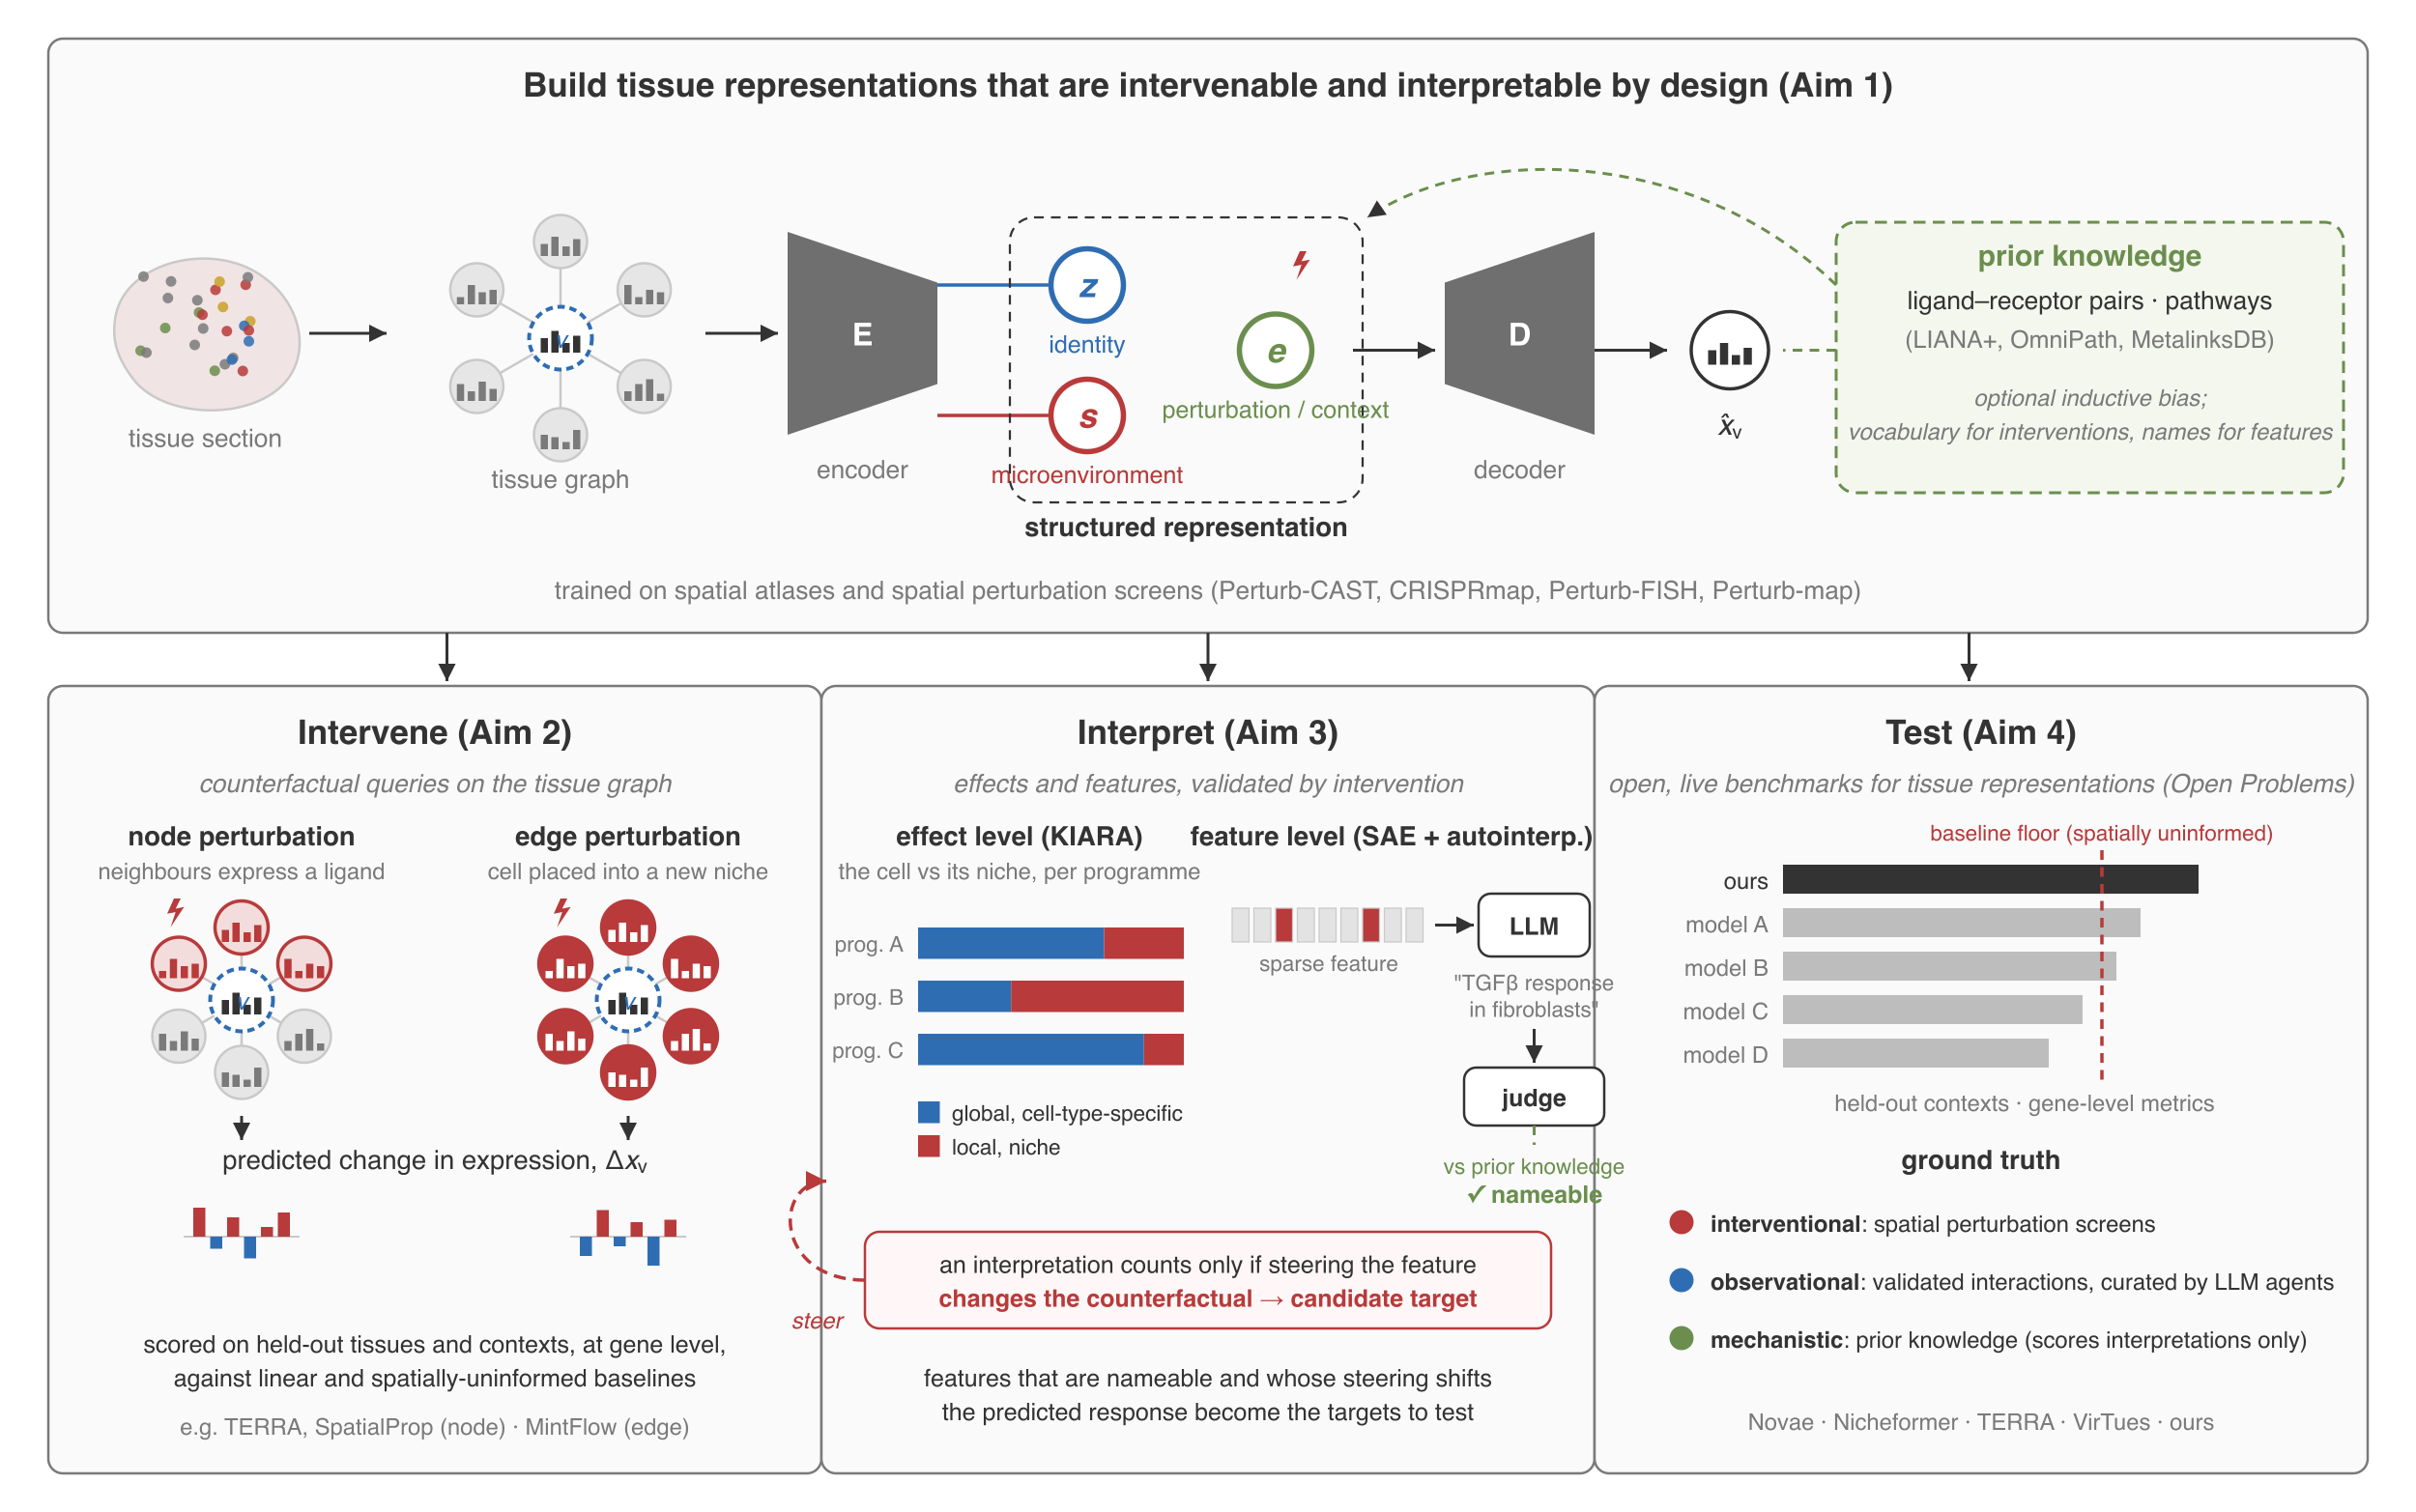
\includegraphics[width=0.82\textwidth]{figures/research_plan_fig1.pdf}
\caption{\textbf{Tissue representations one can intervene on, interpret and test.} \emph{Aim 1:} spatial atlases, spatial perturbation screens, measured cell contacts and agent-curated validated interactions become a benchmark with a spatially-uninformed baseline as its floor. \emph{Aim 2:} two model families are built on these data, decomposable and black-box. \emph{Aim 3:} both answer the same counterfactual queries on a cell's neighbours. \emph{Aim 4:} the first family is read through its structure, the second through its features, and an interpretation counts only if steering it changes the counterfactual.}
\end{figure}

\section{Gather data and build ground truth (Aim 1)}

The bottleneck is not architecture. It is that no dataset can currently falsify a prediction about how a cell responds to its neighbours. The largest spatial corpus reaches 112 million cells, but its gene panels differ from study to study and are absorbed as a batch token, so a gene absent from a panel is indistinguishable from a gene not expressed \citep{birk2026terra}; such atlases cannot adjudicate a ligand--receptor claim. I will therefore start with the data on which both families will be trained and judged, from three sources.

First, interventional ground truth. In vivo and in situ perturbation screens now read perturbation identity and transcriptome-wide phenotype from the same section, so that the response of a perturbed cell and of its unperturbed neighbours are measured together \citep{dhainaut2022perturbmap, gu2025crisprmap, binan2025perturbfish, shen2026spatialperturbseq, baysoy2026perturbdbit, breinig2026perturbcast}, which our perspective singled out as the next step for perturbation modelling \citep{dimitrov2026interpretation}. Second, measured contacts. Enzymatic labelling now records which cells physically interacted in vivo, with a paired transcriptome and without committing to a receptor \citep{pasqual2018lipstic, nakandakarihiga2024ulipstic}; barcode transfer between neighbours coupled to a sender-side CRISPR screen adds a causal layer to the contact \citep{du2026matchseq}; and proximity ligation on adjacent sections gives location-resolved, protein-level evidence for individual ligand--receptor pairs \citep{liu2026cytosignal}. Each gives contact pairs, ligand--receptor identity or tissue coordinates, none gives all three, and none is human; combining them is the work. Third, validated interactions in public data. Language-model agents will curate datasets in which an interaction was experimentally confirmed, extending the agentic curation that now keeps expression repositories current \citep{youngblut2026scbasecount} from expression matrices to validated communication events, with the extraction itself benchmarked so that its biases are measured rather than inherited.

These data become a live benchmark with a spatially-uninformed baseline as a mandatory floor, routed through the Open Problems task I lead \citep{luecken2025openproblems}. This aim succeeds when an external group can score a tissue model on a measured interaction or perturbation response rather than on a prior-knowledge database.

\section{Build tissue representations (Aim 2)}

Interpretability can be engineered into a model or recovered from it, and I will pursue both rather than bet on one. The decomposable family will be staged generative models in which every term is a fitted object: each cell's basal state, the pooled effect of each perturbation in a shared programme space, and only then the residual interactions with cell type and niche, so that an intervention is an operation on a named term rather than a prompt to a black box. The ligand--receptor and pathway layer of LIANA and OmniPath will serve as the vocabulary in which programmes are named and interventions specified \citep{dimitrov2024lianaplus, turei2021omnipath}. Prior knowledge remains an inductive bias, never a requirement: unsupervised disentanglement is ill-posed in general, but biology gives us the priors to make it well-posed in practice \citep{piran2024biolord, dong2025simvi}.

The black-box family will be tissue models of the class the current generation belongs to \citep{birk2026terra, tejadalapuerta2025nicheformer, blampey2025novae}, trained on the Aim 1 corpus without structural constraints, so that the trade between capacity and structure is measured rather than assumed, and Aim 4 has a substrate of our own. I do not intend to compete on the number of cells; I intend to compete on what the representation can be asked.

Both families must answer counterfactual queries on a cell's context and be scored on held-out contexts, at gene level, against linear and spatially-uninformed baselines \citep{ahlmanneltze2025linear, wu2024perturbench}. I have one first model of each kind, Cellina and KIARA, and will develop each into a line, on transcriptomics first and on spatial proteomics once the architectures are fixed \citep{wenckstern2026virtues}.

\section{Intervene (Aim 3)}

A counterfactual query will be the same interface on both families. Node perturbations alter what a cell's neighbours express, as when a ligand is switched on in the cells around it. In Cellina, pathway-targeted neighbour perturbations built from prior knowledge recover their responses \citep{moeed2026cellina}; whether this transfers to the sparse, single-ligand regime experiments actually use is open, so I will parameterize the intervention through the ligand--receptor layer, deleting a ligand in a given sender or dosing a cytokine, so that interventions compose and transfer across tissues. Edge perturbations rewire the neighbourhood itself, placing a cell into a different niche. Existing models attempt both kinds of query \citep{birk2026terra, sun2025spatialprop, akbarnejad2025mintflow}, but none has been validated against measured responses in held-out tissue, which Aim 1 makes possible. Spatial screens have shown that neighbourhood density changes what a knockout does \citep{binan2025perturbfish}; whether a model predicts that change in a tissue it has never seen is the test for this aim.

\section{Interpret (Aim 4)}

The two families require two different readings, and one rule makes either reading count. Decomposable models are read through their structure. KIARA-style decomposition splits an observed in vivo response to a perturbation into a global, cell-type-specific term and a local niche term, with the additive stages fit first. The output is, per perturbation and programme, how much of an effect is the cell and how much its neighbourhood, in the pathway vocabulary my prior-knowledge resources provide \citep{turei2021omnipath, farr2024metalinksdb}.

Black-box models are decoded once trained. I will learn sparse dictionaries over their latents and describe each feature with an autointerpretability pipeline: a language model that sees only activations proposes what a feature encodes, and an independent judge scores that description against prior knowledge and Aim 1 ground truth \citep{bricken2023monosemanticity, templeton2024scaling, paulo2025autointerp}. Sparse autoencoders have begun to expose such features in single-cell and spatial foundation models \citep{pedrocchi2025saescfm, handa2026saffron, kendiukhov2026atlas}. I have built such an LLM-judged benchmark for clinical foundation models (ehrx; conceived and led by me, co-first and corresponding author, in progress) and will port it to tissue. The two lines are orthogonal: decomposition does not require dictionaries and dictionaries do not require decomposition, although I anticipate that dictionaries whose priors are shaped by pathway knowledge will sit between them.

What joins the lines is a rule. An interpretation counts only if intervening on it, steering a dictionary feature or zeroing a fitted term, changes the Aim 3 counterfactual prediction. Features and terms that are nameable and whose perturbation shifts the predicted response are the candidate targets this programme delivers; the fraction that pass this rule, reported against a null, is my measure of success.

\section{Fit and route to the clinic}

Nicheformer and Open Problems were built at the Computational Health Center \citep{tejadalapuerta2025nicheformer, luecken2025openproblems}, and both are the point of contact for Aims 1 and 2. Its groups working from single cells and spatial data towards patients, on tumour neighbourhoods, and on pathology and microscopy images are the partners I envision for translation in two steps: first, a ranked list of interventions whose predicted effect is nameable and holds in unseen contexts; second, patient sections summarized as niche-programme activities and related to outcome and treatment. The first disease setting will be colorectal cancer, where Cellina's cohort and its TGFβ and NFκB/MAPK fibroblast programmes already exist. I bring the LIANA and Open Problems communities, an MSCA fellowship, and a funded CZI collaboration with the Saeys group (VIB--UGent), where I am a named key person; an ERC Starting Grant, for which I am eligible from 2027, will be built on Aims 2--4. Methods papers will go to \emph{Nature Methods} and its sister journals, where my work has appeared, and the general machine-learning problems the programme raises, counterfactual evaluation under distribution shift and identifiability of disentanglement on graphs, to machine-learning venues, where Cellina is under review.

\begin{center}\footnotesize\renewcommand{\arraystretch}{0.9}
\begin{tabular}{@{}p{0.06\textwidth}p{0.20\textwidth}p{0.18\textwidth}p{0.18\textwidth}p{0.20\textwidth}p{0.12\textwidth}@{}}
\toprule
 & Aim 1 Gather & Aim 2 Build & Aim 3 Intervene & Aim 4 Interpret & Group \\
\midrule
Y 1--2 & Screens and contacts assembled; benchmark live & First model of each family & Node and edge queries on both & Decomposition readout; first dictionaries & 2 PhD, 1 postdoc \\
Y 2--4 & Agent-curated interactions & Multi-tissue; proteomics & Held-out-tissue validation & Autointerpretability on tissue; steering rule & +1 postdoc, +1 engineer \\
Y 4--5 & Benchmark used by external groups & Release of both lines & CRC intervention list & Steerable feature and term catalogue & 5--6 members \\
\bottomrule
\end{tabular}
\end{center}

\begin{multicols}{2}\fontsize{8}{9}\selectfont
\bibliographystyle{naturemag}
\bibliography{research_plan}
\end{multicols}
\end{document}
